\section{Introdução}

\begin{frame}

    \frametitle{Introdução - Motivação}
    % neste frame vamos ter que falar que há a oportunidade de reduzir gasto energético em outras partes da produção onde não se gasta energia para esquentar o metal.
    \begin{itemize}
        % \item Aço é essencial para muitas indústrias
        \item Em 2023, estima-se que foram produzidas 1,9 bilhão de toneladas de aço no mundo. \cite{worldsteel.org_2024}
        \item Todas as etapas do processo produtivo de ação são extremamente intensas em gasto energético. O custo de produção de todo esse metal é de aproximadamente 20.99 GJ/ton o que resulta em $39,88\times10^{15}J (Peta)$ no total.
        \item Reduzir o custo energético da produção de metais é essencial para o crescimento sustentável da sociedade global.
    \end{itemize}
\end{frame}

% \begin{frame}{Introdução - Produção de aço}
%     \begin{figure}
%         \centering
%         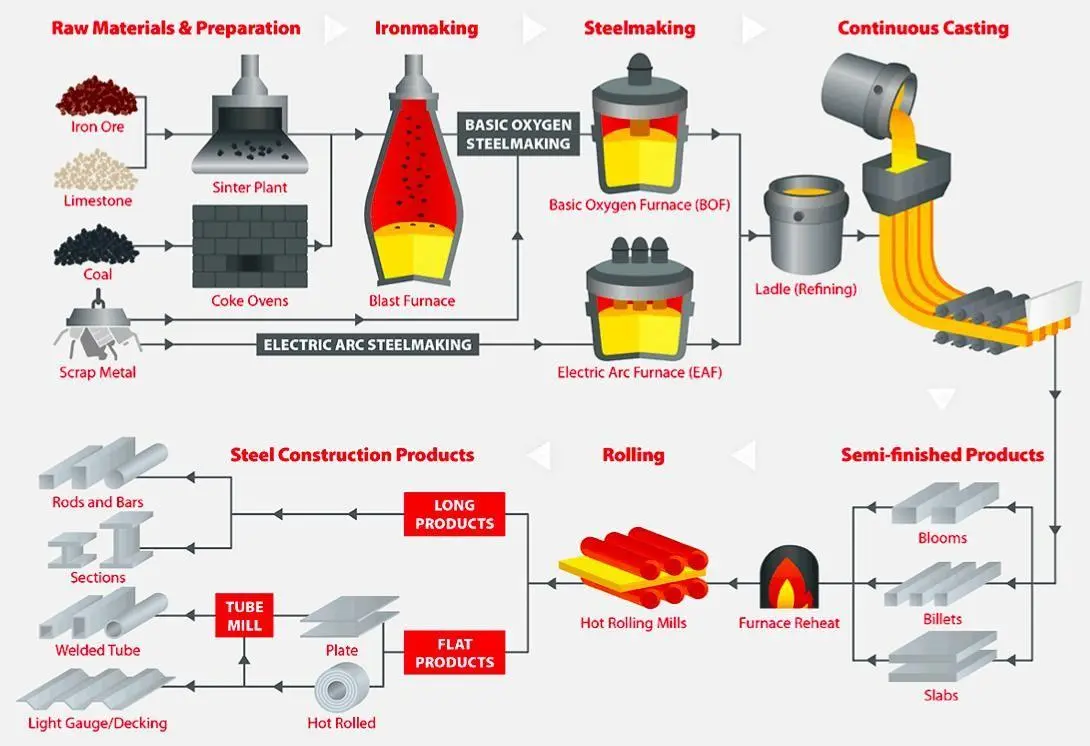
\includegraphics[width=0.55\linewidth]{imagens/ciclo_producao_aco.png}
%         \caption{Ciclo de produção do Aço}
%         \label{fig:ciclo-producao-aco}
%     \end{figure}
% \end{frame}
% \begin{frame}{Introdução - Produção de aço}
%     \begin{figure}
%         \centering
%         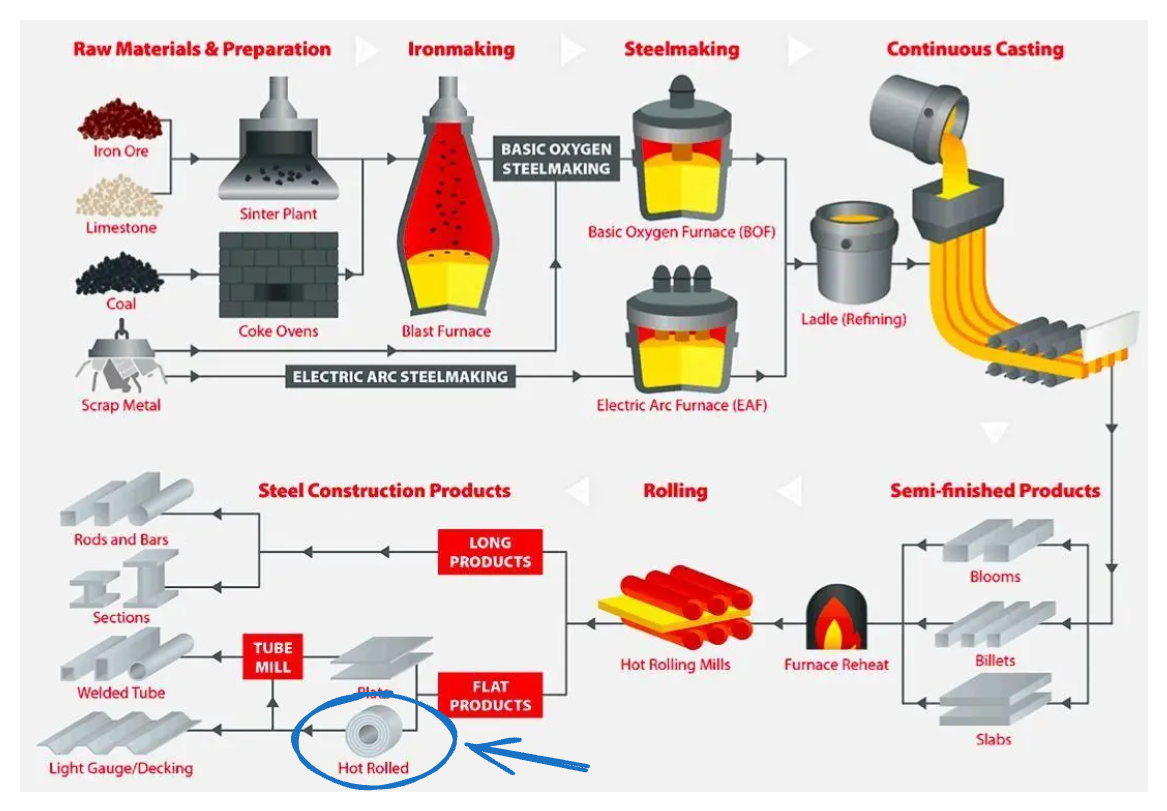
\includegraphics[width=0.55\linewidth]{imagens/ciclo-producao-aco-1.png}
%         \caption{Ciclo de produção do Aço}
%         \label{fig:ciclo-producao-aco-1}
%     \end{figure}
% \end{frame}

\begin{frame}{Introdução - Armazenamento de bobinas quentes}
    \begin{figure}
        \begin{figure}
            \centering
            \includegraphics[width=0.5\linewidth]{imagens/rolled-coils-in-storage.png}
            \caption{Bobinas diferentes em armazenamento}
            \label{fig:bobinas-armazenamento}
        \end{figure}
    \end{figure}
\end{frame}
\begin{frame}

    \frametitle{Introdução - Objetivos}

    \begin{itemize}
        \item Organizar as bobinas em um depósito de forma a minimizar os movimentos futuros e, consequentemente, os gastos energéticos, visando a uma distribuição (\textit{layout}) ótima para atender às demandas previstas.
        \begin{itemize}
            \item Assumimos que conhecemos com antecedência as demandas que devem ser atendidas.
            \item Assumimos plena disponibilidade de maquinário e de pessoal para realizar as movimentações necessárias.
        \end{itemize}
    \end{itemize}
\end{frame}